\chapter{Joint Decisions \who{Dubernet}}
\label{ch:jointtrips}
% ##################################################################################################################

\hfill \textbf{Author:} Thibaut Dubernet

\begin{center} 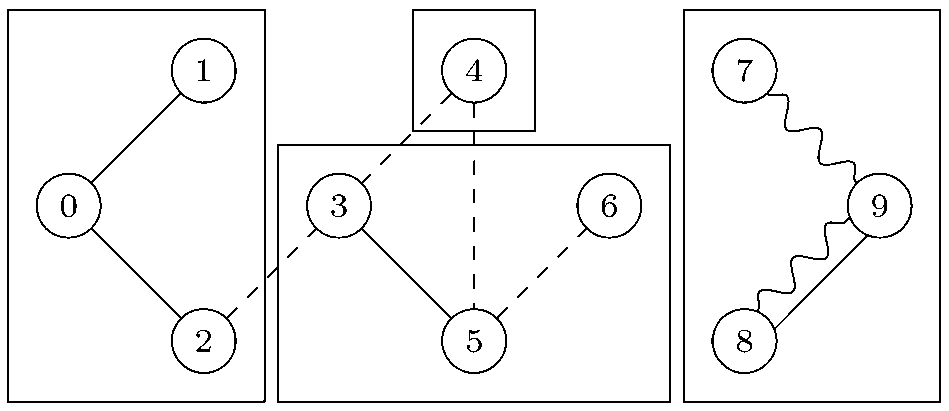
\includegraphics[width=0.4\textwidth, angle=0]{extending/figures/Jointtrips/group.png} \end{center}

% ##################################################################################################################
{ % scope for our commands: do not pollute our little friends

% ##################################################################################################################

\newcommand\authoranddate{\citet}
\newcommand\eg{\emph{e.g.}\xspace}
\newcommand\eg{\emph{i.e.}\xspace}
\newcommand\pudptw{Pick-Up and Delivery Problem With Time Windows\xspace}
\newcommand\structeqmodel{structural equation model\xspace}
\newcommand\ga{genetic algorithm\xspace}
\newcommand\gas{genetic algorithms\xspace}
\newcommand\Gas{Genetic algorithms\xspace}
\renewcommand\matsim{MATSim\xspace}

% Figures crap
\newcommand\insfig[2]{%
	\insfigwidth{#1}{#2}{.8\textwidth}
}
\newcommand\insfigwidth[3]{%
\createfigure{#1}{#1}{}{%
		\includegraphics[width=#3]{extending/figures/Jointtrips/#2}%
		}{}%
}

\newcommand\inssubfigwidth[3]{%
\createsubfigure{#2}{%
		\includegraphics[width=#1]{extending/figures/Jointtrips/#3}%
		}{}{\quad}%
}
\newcommand\inssubfig[2]{%
\inssubfigwidth{.46\textwidth}{#1}{#2}%
}
\newcommand\insfigwithsubfigs[2]{%
\createfigure{#1}{#1}{}{%
		#2%
		}{}%
}

% ##################################################################################################################

This chapter describes the extension of \matsim to consider what we name \emph{joint decisions}.
\cref{sec:td:intro} explains what we name joint decision, and gives an overview of why such processes
are important in transportation.
\cref{sec:td:algo} then presents concepts to model this behavior,
presents a generalisation of the \matsim algorithm to search for solutions to what
we call the \emph{joint planning problem},
and gives technical insights on how this implementation could be achieved,
given the \matsim software architecture.

\section{Joint Decisions and Transport Systems\label{sec:td:intro}}
%!!!!!!!!!!!!!!!!!!!!!!!!!!!!!!!!!!!!!!!!!!!!!!!!!!!!!!!!!!!!!!!!!!!!!!!!!!!!

\subsection{Motivation}
\todo{Shorten this A LOT!!!!}

In recent years, there has been a growing interest in the social dimension of travel,
and how travel decisions are influenced not only by the global state of the transportation system,
but also by joint decisions and interactions with social contacts.

A very active field of research is the study and modeling of intrahousehold interactions
and joint decision making, % \cite{TimmermansZhang_TransResB_2009},
often using the classical random utility framework extended to group decision making.
%
A classical way to cope with the possibly conflicting objectives of different members of the household
is to specify a group level utility function.
%
For instance,
\authoranddate{ZhangEtAl_TransResB_2005,ZhangJEtAl_TRR_2007}
develop a model where time for different activity types is allocated to household members,
subject to time constraints (including equality of time participation in joint activities),
using a group level utility function formulated as a multilinear combination of the individuals'
utilities --- that is, a linear combination of individual utilities and pair-wise
product of individual utilities;
%
% For instance,
\authoranddate{KatoMatsumoto_TransResB_2009}
use a linear combination of the utility functions of the household members as a group utility.
The assumption behind this kind of models is the existence of ``utility transfers'':
individuals accept to decrease their own utility if it allows to increase
the utility of others by a certain fraction of their loss.
%
\authoranddate{BradleyVovsha_Transportation_2005}
focus on the ``daily activity pattern'' generation,
with household ``maintenance'' tasks (\eg shopping) allocation and possibility of joint activities.
To do so, they assume a layered choice structure,
choosing first a daily activity pattern for each member,
and then assigning joint and maintenance activities.
%
\authoranddate{GliebeKoppelman_Transportation_2005} also base their model on the daily activity pattern concept,
choosing first a ``joint outcome'' (the sequence of individual and joint activities),
and then an individual pattern for each household member.
Those models rely on enumeration of the possible household level patterns.
%
\authoranddate{GliebeKoppelman_Transportation_2002}
also derived a constrained time allocation model,
which predicts the time passed by two individuals in joint activities.
Rather than postulating a group level utility function,
the models of those authors specify a special distribution for the error terms of the individuals.
In this setting,
the error term of the individuals are correlated so that the probability
of choosing a given joint output is the same for all individuals.
%
\authoranddate{HoCAndMulley_Transportation_2013} also estimate models in which members of the household
perform choices constrained by the choice of a household level travel pattern.
Their data, as well as the parameters of the models,
show high joint household activity participation on weekends,
and a high dependence of joint travel on trip purpose and household
mobility resources.
Those results highlight the importance of representing joint household decisions,
in particular when going beyond the ``typical working day''.
%
\authoranddate{VovshaGupta_Transportation_2013} formulate a time allocation model for multiple worker households,
which considers a positive utility for members of the household
to be home jointly, as it makes joint activities possible.
The estimation results show a significant influence of this kind of synchronization mechanism.
%
Most models listed in this paragraph
are specific to given household structures;
in particular, separate models need to be estimated for different household sizes.

Household level decision processes have also been modeled with approaches which significantly differ
from the classical random utility framework.
%
\authoranddate{GolobMcNally_TransResB_1997}
propose a \structeqmodel,
which predicts time allocation and trip chaining based on the sociodemographics of a household.
\authoranddate{Golob_TransResB_2000}
also used a \structeqmodel to model the dependency of time allocations
of the two heads (man and woman) of a household.
%

%
Another class of approaches,
more oriented toward multiagent simulation than analysis,
is the use of optimization algorithms to generate households plans.
They handle the household scheduling problem by transforming it into a deterministic utility maximization problem.
Contrary to the previously presented approaches,
those alternatives do not lead to the estimation of a model against data.
%However, the estimation of the utility function is usually not part of those approaches.
%
The first of those approaches was introduced by \authoranddate{Recker_TRR_1995}.
By extending increasingly the formulation of the \pudptw, a well studied combinatorial optimization problem,
he formulates the problem of optimizing the activity sequence of members of a household
as a mathematical programming problem.
%taking into account vehicle constraints, individual and household level activity,
%possibility of choosing whether to perform or not an activity, with the possibility of shared rides.
However, due to the complexity of the problem,
the full problem cannot be solved exactly by standard operations research algorithms,
and the activity durations are not part of the optimized dimensions.
\authoranddate{ChowRecker_TranResB_2012} designed an inverse optimization method
to calibrate the parameters of this model
%, including the time window constraints,
using measured data.
Also, the formulation from \authoranddate{Recker_TRR_1995}
was later extended by \authoranddate{GanRecker_TransResB_2008}
to introduce the effects of within day rescheduling due to unexpected events.
%
Another attempt to generate plans for households uses a \ga,
building on a previous \ga for individual plan generation
\cite{CharyparNagel_Transportation_2005,MeisterEtAl_Transportation_2005}.
This algorithm optimizes sequence, duration and activity choice for a household,
rewarding the fact that several members of the household perform the same activity
simultaneously, in the way also used by \authoranddate{VovshaGupta_Transportation_2013}.
%
Finally, \authoranddate{LiaoFEtAl_Transportation_2013} formulate the problem of creating
schedules for two persons traveling together as finding the shortest path
in a ``supernetwork'', and solve this problem using exact shortest path algorithms.
They however note that their model is specific to the two person problem,
and that extension to larger numbers of agents may prove to be computationally expensive.
%
%Finally, Fang \emph{et al.} optimize location and time of joint activities, constrained to time windows in pre-determined individual plans, using a multi-objective \ga \cite{Fang2011}.
All those approaches remained experimental,
and were not integrated into multiagent simulation tools.

Another class of methods aiming at multiagent simulations
is constituted rule based systems,
which use heuristic rules to construct household plans.
%
\authoranddate{MillerEtAl_Transportation_2005} develop such a model for household mode choice.
The main difference with an individual mode choice model is the consideration of household level vehicle allocation.
In their model, individuals first choose modes individually.
If a conflict occurs, the allocation that maximizes the household level utility is chosen.
The members which were not allocated a vehicle will fall back on their second best choice,
and/or examine shared rides options.
%
\authoranddate{ArentzeTimmermans_TransResB_2009}
develop a rule base model which
relies on a simulated bargaining process within the household.
Though such models can easily represent complex decision processes,
their calibration and validation is cumbersome.

Other authors have investigated the role of more general social networks on travel.
One of the main incentives to conduct such studies comes from the continuous increase of the share of
trips which are performed for leisure purpose \cite{SchlichEtAl_TransportRev_2004,Axhausen_DonaghyEtAl_2005}.
This fact represents a challenge for travel behavior modeling,
as those trips are much more difficult to forecast than commuting trips:
they are performed more sporadically, and data about those trips is much more difficult to collect
--- in particular concerning attributes of locations and events,
which are needed to make models that do not only consist of random noise.
Understanding better how destination choice for leisure trip is made is therefore essential to improve
the accuracy of those forecasts.

Various studies have been conducted with the idea that an important factor in leisure trip destination
choice, or activity duration choice, is the ability to meet social contacts.
Examples of empirical work include \authoranddate{CarrascoJAHabib_IATBR_2009}; \authoranddate{HabibCarrascoJA_TRR_2011} or \authoranddate{MooreJEtAl_Transportation_2013}.
All those studies show a substantial influence of social contacts on the spatial and temporal
distribution of activities.
%
Based on an analysis of social network involvement and role, \authoranddate{DeutschGoulias_Transportation_2013}
advocate considering the \emph{role} individuals play in different social networks.
Using latent class cluster analysis models to analyse the role of individuals in
the various social networks they are involved in,
they find that ``the decision-making role of an individual can differ vastly across different
social engagement types''.
%
\authoranddate{Frei_PhDThesis_2012} demonstrated in a simulation experiment how considering social interactions
in leisure location choice can help increase the accuracy of predicted leisure trip distance distribution.

Another field of empirical research studies the spatial characteristics of social networks.
For instance, \authoranddate{CarrascoJAEtAl_TRR_2008} studied the relationship between individual's socioeconomic
characteristics and the spatial distribution of their social contacts.
This kind of empirical work allows to specify and estimate models able to generate synthetic social networks,
given sociodemographic attributes and home location.
An example of such a model, based on the results of a survey in Switzerland,
can be found in \authoranddate{ArentzeEtAl_TRB_2012}.
This kind of model is essential if one wants to include social network interactions
in microsimulation model.

This integration of social networks in multiagent simulation frameworks has already
been attempted by other authors.
Due to their disaggregated description of the world,
such models are particularly well suited to the representation of complex social topologies.
\authoranddate{HanQEtAl_TransResPartA_2011} present experiments of using social networks
to guide activity location choice set formation in the FEATHERS multiagent simulation framework.
Using a simple scenario with 6 agents forming a \emph{clique},
%(a network where all agents have social ties with all other agents),
they consider the influence of various processes like
information exchange and adaptation to the behavior of social contacts to increase the probability
of an encounter.
They do not, however, represent \emph{joint decisions}, such as the scheduling of a joint activity.
The same kind of processes have been investigated by \authoranddate{Hackney_PhDThesis_2009},
using more complex network topologies,
within the \matsim framework, used in this paper.
\authoranddate{RonaldEtAl_TransResB_2012}
and \authoranddate{MaEtAl_TRR_2011,MaEtAl_IATBR_2012}
present agent based systems which do integrate
joint decision making mechanisms,
based on rule based simulations of a bargaining processes.
They are not yet integrated into
any operational mobility simulation platform.

% intro mon boulot
Building on all those ideas,\todo{lesquelles? preciser limitations identifies
et comment l'approche presente resoud tout}
the work presented in this paper aims at including explicit coordination of individuals
in a multiagent simulation software framework.
A game-theoretic model of joint decisions for daily planning is introduced,
and a simulation algorithm implemented using the
\matsim software framework.
The process is designed to be able to handle complex social network topologies,
%but the current implementation is restrained to a network consisting of
%isolated \emph{cliques}.
%Such a network is a good abstraction for the network of intrahousehold relationships,
%which importance should be clear from the review above.
but the current study focuses on intrahousehold ties only.
The results of an implementation for intrahousehold ridesharing
for a scenario for the Zurich area, Switzerland, are analyzed.
Comparing the results of this scenario with travel diary data,
limitations of the current implementation are identified,
and directions for future work are sketched.

\subsection{The Joint Planning Problem}

\section{An Solution Algorithm for the Joint Planning Problem: a Generalization of the MATSim Process\label{sec:td:algo}}
%!!!!!!!!!!!!!!!!!!!!!!!!!!!!!!!!!!!!!!!!!!!!!!!!!!!!!!!!!!!!!!!!!!!!!!!!!!!!

\subsection{Algorithm}
%---------------------------------------------------------------------------

Given this theoretical framework, one needs to design and implement an
algorithm to search for allocations of daily plans to individuals, that
satisfy this solution concept.

This section presents the EUNOIA implementation, which was build using
the MATSim software framework. This implementation consists of two
groups of components:

\begin{enumerate}
\item
  A \emph{Controller} that implements the extension of the MATSim
  co-evolutionary algorithm, outlined hereafter. It is implemented in a
  modular fashion, to be easily adapted to the specific need of
  different simulation scenarios
\item
  Specific implementations of the modular components, to test the
  behavior of the approach and apply it to the case studies.

  \begin{enumerate}[i)]
  \item
    data structures to represent households and generic social networks
    were implemented, as well as the ways to identify groups for
    replanning
  \item
    specific replanning modules to explore the set of possible joint
    decisions were implemented
  \end{enumerate}
\end{enumerate}

The solution algorithm and implementation is a generalization of the
MATSim process presented in the introductory session. The following
sections outline the different elements implemented in the EUNOIA
project.

\paragraph{Controller}

The MATSim framework provides a \emph{Controller} to build and configure
co-evolutionary algorithms, where agents each optimize their plan given
the (evolving) state of the transport system.

Unfortunately, this approach makes choices of agents independent ---
which of course goes against the simulation of \emph{joint decisions}.
To be able to implement an algorithm searching for states without
blocking coalitions, one needs a way to represent the influence of
explicit coordination on the utility of a daily plan. This is solved by
including \emph{joint plans} constraints. A joint plan is a set of
individual plans executed simultaneously. Different copies of the same
individual plan can be part of different joint plans --- for instance an
agent might go to a given restaurant alone, with members of its
household or with a group of friends. The score of the different copies
will take into account the influence of the joint plan to which it
pertains. Those joint plan constraints are included using heuristic
rules, applied after mutation operators are applied, and are classified
as strong or weak constraints --- weak constraints are considered when
selecting plans for execution, but are allowed to be broken when merely
selecting plans for mutation. They are then part of the evolution
process. In the current application, the heuristic rules consist in
joining newly created plans with joint trips (strong) or with leisure
activities at the same location at the same time (weak).

To allow handling joint plans, replanning needs to be performed for
groups of agents. This is straightforward for households: all agents of
a same household are always handled as a single group. For more general
social networks, agents are handled with all agents with whom they have
a joint plan, plus some social contacts with whom new joint plans can be
created. Details are presented in the ``Implementation'' section.

For each group, two actions are then possible. For most groups, an
allocation of existing plans, fulfilling the joint plans constraints, is
selected for execution. Based on plan scores, randomized by adding an
extreme value distributed error term, an allocation without improving
coalitions is searched for by an algorithm inspired by the ``Top Trading
Cycle'' algorithm used for the House Allocation Problem
\cite{SchummerVohra_NisanEtAl_2007}.

For the other groups, a plan allocation is selected and copied. The
copied plans then undertake mutation, to make the agents explore new
alternative joint plans. What kind of mutation is performed determines
which alternative plans will be tried out by the agent. The modules
currently implemented are presented in the ``Implementation'' section.

Agents have a limited memory size, keeping at most 3 plans per joint
plan composition, and 10 plans in total. If this limit is exceeded, one
should keep the plans which have the highest probability to create
improving coalitions, that is, to be preferred to the other plans in the
agent's memory. To this end, a lexicographic ordering is used: the
process removes the joint plan which maximizes the number of individual
plans which are the worst of the agents' memories. If several joint
plans have the same number of worst plans, the process chooses among
them the joint plan which maximizes the number of second worst plans,
and so on until the ``worst'' joint plan is unique. When the overall
maximum number of plans in the memory of an agent is reached, the worst
individual plan for this agent is removed along with plans of other
agents of the same joint plan. Each agents keeps at least one plan not
part of a joint plan, as there may otherwise not be any state without
blocking coalitions. Agents are parsed in random order, to avoid the
emergence of ``dictators'' over iterations, whose worst plan would
always be removed, even if it is the only ``bad'' plan of a joint plan.

Though those selection operators seem to be in accordance with the
chosen solution concept, it is difficult, if not impossible, to prove
that the process will actually converge towards the state searched. As
noted by \cite{FiciciEtAl_ITEC_2005}, when they perform a theoretical
analysis of different selection methods in a co-evolutionary context,
``Co-evolutionary dynamics are \emph{notoriously complex}. To focus on
our attention on selection dynamics, we will use a simple evolutionary
game-theoretic framework to eliminate \emph{confounding factors} such as
those related to genetic variation, noisy evaluation, and finite
population size''. Those ``confounding factors'' can however not be
eliminated from an actual implementation of a co-evolutionary algorithm,
and rigorously proving that a given algorithm actually implements a
specific solution concept is very tedious, if not impossible.

With iterations, agents build a choice set of daily plans that becomes
better and better given the actions of the other agents. However, the
presence of a large portion of agents with plans resulting from random
mutation creates noise, not only for the analyst looking at the output
of the simulation, but for the agents themselves when they compute the
score of their plans. To solve this issue, when the system reaches a
stable state, agents stop performing mutation, and only select plans
from their memory for 100 iterations, using the absence of improving
coalition with randomized scores. This ensures that the selected plans
are the result of a behavioral model, rather than the result of random
mutation operators.

\subsection{Technical Considerations on the Implementation}
%---------------------------------------------------------------------------
As highlighted in \cref{ch:extensionpoints},
the preferred way to add new behaviors to the \matsim software is
by designing \emph{pluggable} elements,
that can be added to a \emph{Controler} from a configuring ``script''.
\todo{check that \cref{ch:extensionpoints} actually phrases it so\ldots}

This modular approach works well in most of the use cases,
and makes it possible to combine different elements to design highly
specific runs.
There is however something that one can not modify this way,
that is: the general form of the evolutionary process.
This process is exactly what has to be modified to include joint decisions
--- 
this section focuses on the challenges and solutions to undertake such major
modification, for reference from developers facing this exact problem\todo{reformulate that}.

The one important modification of the process is that in the standard \matsim process,
\emph{replanning} is performed independently for each agent,
whereas for joint decisions agents have to be replanned \emph{as groups}:
selection of plans needs to fulfill \emph{joint plan constraints}
and is performed using the group-level ``absence of improving coalition''
criterion, and mutation operators are allowed to work on several plans at the same time,
for instance to insert \emph{joint trips}, or select the location of a
\emph{joint activity}.

Doing so requires the replacement of the \emph{replanning listener},
that is, the element responsible of managing the whole replanning step.
This can only be done by implementing a separate controller.\todo{say better}

Modularity was kept as high as possible, in particular by providing standard ways
to use the default individual-based replanning modules from this new element.

\section{Selected Results\label{sec:td:results}}
%!!!!!!!!!!!!!!!!!!!!!!!!!!!!!!!!!!!!!!!!!!!!!!!!!!!!!!!!!!!!!!!!!!!!!!!!!!!!
\subsection{Joint Travel and Activities with Leisure Contacts}
%---------------------------------------------------------------------------
\insfigwithsubfigs{Share of Passenger Trips Per Purpose}{%
	\inssubfig{Simulation}{passenger-per-type-ju3-asShareOfPassengerTrips}%
	\inssubfig{National Travel Survey}{passenger-per-type-MZ-asShareOfPassengerTrips}%
}

\insfigwidth{Travel Distance to Leisure Activities}{distance-bxp-purpose}{.6\textwidth}

\subsection{Joint Travel within Households}
%---------------------------------------------------------------------------

\section{Further Reading}
%!!!!!!!!!!!!!!!!!!!!!!!!!!!!!!!!!!!!!!!!!!!!!!!!!!!!!!!!!!!!!!!!!!!!!!!!!!!!
The work presented in this chapter has been described in more details in various papers.
\authoranddate{DubernetAxhausen_TransLett_2013}
presents an early stage of the algorithm, applied to a toy scenario.
%\authoranddate{DubernetAxhausen_unpub_Frontiers_2013}
%\authoranddate{DubernetAxhausen_unpub_SmartCities_2013}
\authoranddate{DubernetAxhausen_STRC_2014}
compares gives more theoretical ground,
by making more explicit reference to game theory,
and compares two \emph{solution concepts} for
the solution of the joint planning problem in the household case:
the absence of improving coalition presented here,
as well as a ``joint utility'' formulation,
classical in the literature.
\authoranddate{DubernetAxhausen_Transportation_forth}
presents a validation of the model for the household case,
using a Zurich scenario.

} % close scope: all our personal commands are gone (hopefully...)
